% $Id: AllegProposal.tex,v 1.8 2000/07/05 21:02:12 culver Exp $
% AllegProposal.tex
% by A. Thall
% 13. Feb 2003
%
% Small edits and a few additions made by R. Roos
% 21 Jan 2007
% Most particularly, the "box" around the thesis statement has been removed,
% section titles have been modified. The section named "Prior work II" has
% been commented out. The \topmargin has been changed to -.5in and the
% change to \parindent has been commented out.
% The filename "nausicaa.eps" has been changed to simply "nausicaa" so that
% pdflatex can be used on the file (and a file named "nausicaa.pdf" has
% been created using the "epstopdf" command).
% Several subsections have been added to illustrate subsection usage.
% The word "comp" has been replaced by "project" or "thesis" throughout.
% Other small changes have been made.
%
% This document provides a sample Senior Project Proposal template for use
% by students in Allegheny's CS and Applied Computing programs.

\NeedsTeXFormat{LaTeX2e}
\documentclass[11pt]{article}

%The following is used by WinEdt to set up cross-referencing to the BibTeX files
%It is NOT commented out---the comment lets it be simply ignored by non-WinEdt LaTeX compilers

%GATHER{mybibtexDB.bib}

\usepackage{setspace}
\usepackage{amsmath}
\usepackage{amssymb}
\usepackage{epsfig}
\usepackage{fancybox}
\usepackage{listings}
\usepackage{algo}
\usepackage{url}
\usepackage{indentfirst}

\setlength{\textheight}{9in}
\setlength{\textwidth}{6in}
\setlength{\oddsidemargin}{.25in}
\setlength{\topmargin}{-.5in}  % changed from -.25 by RSR on 1/21/07
%\parindent .5in    % commented out by RSR 1/21/07

%put words in the hyphenation statement if you want to enforce
%how LaTeX should break them (or not) at the end of a line.
%\hyphenation{repre-sen-tations problems exact linear}
\hyphenation{itself}

%%%%%
%% Commented out -- RSR, 1/21/07
%%%%%
% The following provides a box to surround the thesis statement
%\newenvironment{Thesis}%
%{\begin{Sbox}\begin{minipage}{.95\linewidth}}%
%{\end{minipage}\end{Sbox}\begin{center}\fbox{\TheSbox}\end{center}}

\title{A Hybrid Execution Model for a Runtime System to Execute Integration Processes for Business Intelligence in the Cloud \\ Proposal thesis}
\doublespace
\author{Daniela F. Sellaro \\ Thesis supervisor: Dr. Rafael Z. Frantz}

\begin{document}

% You can specify a language and other options for
% the code-formatting "listings" package
\lstset{language=C++,basicstyle=\small,
        stringstyle=\ttfamily,showstringspaces=false}


\singlespace
\maketitle

\begin{abstract}                % ~350 words max
Companies are taking advantage of cloud computing to improve their business processes. The cloud computing requires the interaction with many kinds of applications, so it is necessary to improve the performance of software tools that allow keeping information on all these applications consistent and synchronised. Integration platforms are specialised software tools that provide support to design, implement, run, and monitor integration solution. The runtime system is the part of the integration platform responsible for running integration solutions.
Integration platforms, available as iPaaS services, consist of the same platforms designed and implemented for use on on-premise applications, merely encapsulated with a web interface and a few new adapters for connecting applications to the cloud or with cloud services. Therefore, runtime systems need to be adapted to the context of cloud computing, mainly seeking an increase in its performance and an optimization of the consumption of computational resources. 
This proposal presents a survey, based on comparison framework, which analyses integration platforms from the runtime system perspective, taking into account two dimensions of properties that allow comparing their capacity to process messages efficiently and to ensure a fair execution of tasks. Thus, we indicate the research directions, which will be addressed in our doctoral thesis and will contribute to migrate and adapt integration technologies to the context of cloud computing.
\end{abstract}
%
% This sets section-numbering to only include Section and Subsection numbers
\setcounter{secnumdepth}{3}
%
\newpage
\doublespace
%
% Identification.tex
%==============================================================================
\section{Identification info}
\label{sec:identification}
%==============================================================================

\subsection{Name}
Daniela Freire Sellaro
\subsection{Thesis supervisor}
Dr. Rafael Zancan Frantz 
\subsection{Joint supervisor}
Dr. Inma Hernández 
\subsection{Research line}
Computational Modelling, Optimization and Systems Control
\doublespace

% Introduction.tex
%==============================================================================
\section{Introduction}
\label{sec:introduction}
%==============================================================================

%-- Context
\noindent 
Companies often need to use their software ecosystems~\cite{messerschmitt:2005} to support and improve their business processes. These ecosystems are composed of many applications, usually designed without taking into account their possible integration. Within the area of Software Engineering, the field of studies known as Enterprise Integration Applications (EAI)~\cite{frantz2016} seek to provide methodologies, techniques and tools for the design and implementation of integration solutions. In general terms, an integration solution aims to orchestrate a set of applications to keep them synchronized or provide new features that can be built from those already developed. An integration solution is composed of processes that contain the integration logic and ports that encapsulate adapters for communication protocols, which connect ecosystem processes or applications to the integration solution.

Integration platforms are specialised software tools that provide support to design, implement, run, and monitor integration solution. 
In the last years, many integration platforms have been created by the EAI community. These platforms have been heavily influenced by the catalogue of conceptual integration standards documented by Hohpe and Woolf~\cite{hohpe2004} and adopt the architectural style of pipes-and-filters~\cite{alexander1977}. In an integration solution, pipes represent message channels, and filters represent atomic tasks that implement a concrete integration pattern to process encapsulated data in messages. The adoption of this architecture allows to unsynchronised the tasks that make up the integration solution.

There are several open source platforms that can be used to build integration solutions such as Mule~\cite{dossot2014}, Camel~\cite{isen2010}, Spring Integration~\cite{fisher2012}, Synapse~\cite{rademakers2008,jayasinghe2011}, Fuse~\cite{russell2012}, ServiceMix~\cite{konsek2013}, Petals~\cite{surhone2010}, Jitterbit~\cite{russell2012_1}, WSO2 ESB~\cite{indrasiri2016} and Guaraná~\cite{frantz2012}. Usually, these integration platforms provide a domain-specific language, development toolkit, test environment, monitoring tool, and runtime system. The domain-specific language is focused on the elaboration of conceptual models for the integration solution, with a level of abstraction close to the domain of the problem. The development kit is a set of software tools that allows the implementation of the solution, that is, the transformation of the conceptual model to the executable code. The testing environment allows testing individual parts or the entire integration solution, with the aim of identifying and eliminating possible defects in the implementation of the same. The monitoring tool is used to monitor, at runtime, the operation of the integration solution and detect errors that may occur during message processing. The runtime system provides all the support required to run these integration solutions.

Cloud Computing~\cite{NIST:2011} is another field of research that has drawn the attention of the scientific community and represents a new paradigm of development, commercialization and use of software. This field has been transforming the current software ecosystems and revolutionizing the way companies provide computer support to their business processes. Cloud computing enables companies to contract service packages by dramatically reducing their total cost of ownership (TCO) with the information technology (IT) infrastructure, without sacrificing the quality of the IT support provided to their business processes. This is due mainly to the pay-as-you-go charging model that allows users to rate cloud computing based on the amount of computing resources consumed~\cite{buyya:2009,SOUSA:2009}. Along with the pay-as-you-go model, cloud computing has also brought the elasticity feature, which allows for incremental and decreasing computational resources to better meet the demands of applications running on the cloud infrastructure~\cite{DIAS:2015}.
The advancement of cloud computing technologies has led companies to a major transformation in their software ecosystem, which now includes on-premise applications, migrated applications for virtual machines in the cloud, social media applications and many other software services available in the cloud. 

%-- What is the problem? 
The quality of service that integration solutions are able to achieve in terms of message processing, is directly related to the runtime system the integration platform. Typically, in order to achieve the desired quality of service with an integration solution, software engineers have increased computational resources in the server machine on which the integration platform is installed within the enterprise. This approach links the increased performance of an integration solution to the increase in financial costs required to augment the current hardware or the purchase of a new server with greater processing power that can generate the desired impact on the performance of the runtime systems, thus increasing the number of messages processed by the integration solutions.
The hiring of virtual machines in the cloud to host the integration platforms allows a reduction of the total cost of ownership for the realization of the EAI by the companies, as well as through the feature of elasticity of the cloud, a greater flexibility for the increment of computational resources.

This in itself has led companies to want to migrate integration platforms and run their integration solutions in the cloud. The migration of integration platforms to virtual machines in the cloud has given rise to a new service model that is being referred to by the EAI community as integration Platform-as-a-Service (iPaaS)~\cite{pezzini2011}. Data from 2015 show that, together, Latin America, Central America and North America account for 67\% of the market for iPaaS integration platforms, followed by Europe, the Middle East and Africa, which together account for 22\%, and Asia and the Pacific with 11\% of this market, and these values should remain, with little oscillation, by the end of 2019~\cite{sharma2015}. The traditional market for integration platforms used on-premise registered growth of less than 10\% in 2016, while the market for iPaaS integration platforms had a 60\% expansion over the previous year, representing a global market of 700 million Dollars~\cite{guttridge2017}. As early as 2017, two out of three application integration projects are developed directly with cloud integration platforms~\cite{pezzini2015}. The investment made by companies in iPaaS integration platforms will increase by 40\% by 2019~\cite{sharma2015}, making iPaaS the preferred integration platform by companies and with annual revenue growth higher than the traditional platform market Of integration used on-premise~\cite{guttridge2017,sharma2017}.

%-- % %-- Why it is a problem?
Given the high investments in iPaaS integration platforms, a research effort is needed to study and adapt these platforms to the new paradigm that represents cloud computing. In this context, the efficiency of runtime systems is fundamental since a number of computing resources in the cloud follows the pay-as-you-go model, and therefore has a direct impact on the financial cost involved in executing the solutions. The higher the efficiency of runtime systems, the less computational resources will need to be contracted or consumed in order for an integration solution to achieve the expected quality of service. In this article, performance is defined as the ability to process more messages per unit of time, without having to increase the number of computational resources allocated to the runtime system.

% %-- Our solution
In this proposal, we list ten properties of the runtime systems of integration platforms, divided in two dimensions,  that allow to evaluate the ability to process messages efficiently and ensure a fair execution of tasks. We evaluate theses proprieties in runtime systems of popular integration platforms and we observe that they are not sufficiently adapted to the context of the cloud computing. Based on this survey, we present research directions, that will contribute to migrate and adapt integration technologies to this context.

The rest of this article is organised as follows: Section~\ref{sec:statement} presents the thesis statement and research objectives; Section~\ref{sec:priorwork} presents prior work and current art; Section~\ref{sec:methodology} presents the methodology; Section~\ref{sec:survey} presents our survey, describing the dimensions and their respective properties from which we have revised the integration platform and the issues to investigated derived them; Section~\ref{sec:validation} reports how results will be judged and interpreted; Section~\ref{sec:schedule} shows a time-table for achieving key objectives, and plans in cases where goals are not met by specific target dates; and, finally, Section~\ref{sec:conclusions} presents the concluding remarks.

% \begin{itemize}
% \item
% the thesis statement and research objectives;
% \item
% prior work and current art---other approaches to the problem and
% their drawbacks;
% \item
% methodology and experiment---including background research
% to be done, necessary equipment and algorithmic techniques, and general
% plan-of-attack;
% \item
% analysis and validation---how results will be judged and interpreted;
% \item
% a time-table for achieving key objectives, and one or more fall-back plans
% in cases where goals are not met by specific target dates;
% \item concluding remarks.
% \end{itemize}
\doublespace
% \section{Introduction}\label{ch:overview}

% Creation of a formal research proposal is a daunting task; while authors
% such as Zobel~\cite{zobel:97} discuss the basic mechanics of technical
% writing, and writers such as Griffith et al.~\cite{griffiths:97}
% explain the basics of using \LaTeX\ for such writing, there is little
% guidance on the actual structure of a research proposal.
% This structure may vary considerably depending on the nature of the
% research topic---whether it consists of a coding project, a theoretical
% study, a literature survey or other acceptable topics. Despite their
% differences, all proposals share common features, and this paper provides
% a \LaTeX\ template suitable for most such projects. It is expected that
% a user will modify this template according to the specifics of the
% proposed research; in particular, boiler-plate section headings
% and subheadings should be replaced by informative ones specific to
% the topic.

% \subsection{Components of a Proposal}
% The introduction of a proposal typically acquaints the reader with
% the nature of problem being addressed and the basic idea of the
% project being proposed to address it.  It should hit many of the points
% of the abstract while giving more of the motivation and need for the
% work being proposed.  It should then lay out the structure of the
% paper, telling the reader what will be found in the sections which
% follow.  Thus, the next sections should address the following topics:
% \begin{itemize}
% \item
% the thesis statement and research objectives;
% \item
% prior work and current art---other approaches to the problem and
% their drawbacks;
% \item
% methodology and experiment---including background research
% to be done, necessary equipment and algorithmic techniques, and general
% plan-of-attack;
% \item
% analysis and validation---how results will be judged and interpreted;
% \item
% a time-table for achieving key objectives, and one or more fallback plans
% in cases where goals are not met by specific target dates;
% \item concluding remarks.
% \end{itemize}
% The proposal should also include a bibiography/reading-list.  In
% this case, it is permissible to include references which are not directly
% cited in the text.  (You can use the \verb+\nocite{*}+ command before the
% bibliography section, as below, to include all Bib\TeX\ references
% from a database file in the bibliography.)  You should still cite
% references in the text as appropriate.

% \section{Prior Work}

% Depending on the nature of the topic, prior work should either precede
% or follow the thesis statement.  Some topics will require the
% background information to put the thesis proposal in context.  Others
% are best served by giving the thesis statement first and then contrasting
% and comparing it with prior work in the field.

% \subsection{\TeX}
% If this were a real proposal dealing with how to write proposals,
% it might be appropriate to say a few words
% about Knuth, inventor of the \TeX\ typesetting language \cite{knuth:84}.
% Description of Knuth's contribution goes here.

% \subsection{\LaTeX\ (Lamport, 1984)}
% Description of Lamport's contribution \cite{lamport:94} goes here.

% \subsection{Other Work}
% Description of other contributions leading up to this thesis goes here,
% e.g., Zobel's book on writing for computer science \cite{zobel:97}.

% \section{Thesis}

% It is difficult for students to begin a proposal without an adequate guide;
% my project, therefore, will demonstrate the following thesis:
% %\begin{Thesis}
% \singlespace
% \begin{quote}
% It is both simple and useful to provide students with a \LaTeX\ template
% for their formal thesis proposals.  This will result in far fewer
% questions from students uncertain as to what belongs in their proposals.
% Such a template will be of benefit to students in Computer
% Science/Applied Computing as well as to any others willing and able
% to use \LaTeX\ for their work.
% \end{quote}
% %\end{Thesis}
% \doublespace

% A formal thesis statement should be a \emph{falsifiable} statement about
% the goal you will attempt to achieve with your research project.
% For a purely scientific project, this is the hypothesis you are testing
% with your research.  For an applied programming project, it is usually a
% statement about the feasibility and correctness of your approach and
% the advantages it has over other approaches.  For a survey or study,
% it is usually a statement regarding the need or usefulness of such
% a study, its intended audience, and so on.

% Often, you may want to include an itemized list of goals you plan to
% achieve.  Thus, this paper has the goals of
% \begin{itemize}
% \item
% helping students, by ridding their minds of confusion;
% \item
% helping faculty, too, by eliminating their need to say ``No, no, no!
% You need to include a section on \emph{bleh} and \emph{blah}!
% I told \emph{everybody} that.  I thought I told everybody that.  Arrgghh!!!''
% \end{itemize}
% In summary, this section gives the main idea of what you propose,
% with the goals and contributions it will make to the field; the
% details of proposed implementation and methodology will be given later
% in Sec.~\ref{sec:implem}.

% %\section{Prior work II:  advantages of the proposed work over other approaches}

% If you didn't already discuss prior work, this is a good place to do so.
% %You might include these remarks, if brief, in the preceding section.

% \section{Implementation and Methodology}\label{sec:implem}

% Here, you should lay out the details of how you propose to solve the
% problem and otherwise conduct the research necessary to support your
% thesis.  Include details regarding hardware and software you will use,
% resources you will draw on, algorithms you will implement, and other
% ideas about how you will accomplish your task.  It is inevitable that
% your final work will deviate from earlier plans, as you research your
% topic, learn new methods, and discover what works as expected.

% \subsection{Using Tables and Figures}
% Use tables and figures as appropriate; a picture can explain a lot
% in very compact form, and can keep readers interested.  Avoid things
% that are merely flash and do not
% \begin{figure}
% \centering
% \begin{tabular}{l l l}
% \epsfxsize=1.8in\epsffile{Nausicaa} &
% \epsfxsize=1.8in\epsffile{Nausicaa} &
% \epsfxsize=1.8in\epsffile{Nausicaa} \\
% \end{tabular}
% \caption{Include images in a proposal as appropriate}\label{fig:nausicaa}
% \end{figure}
% add any relevant information.  (See Fig.~\ref{fig:nausicaa}.)

% \subsection{Working with Code and Pseudocode}
% If you have source code to include, you can do so using the
% \emph{listings} package,
% which will format short inline code fragments such as

% \singlespace
% \begin{lstlisting} {}
% for (int i = 0; i < n; i++)
%     cout << "It's easy to add source code to LaTeX documents";
% \end{lstlisting}
% or simply using the \emph{verbatim} environment, which gives a Courier font to literal text:
% \begin{verbatim}
% for (int i = 0; i < n; i++)
%     cout << "It's easy to add source code to LaTeX documents";
% \end{verbatim}
% \doublespace
% The listing environment is good for longer code examples and for use in figures,
% such as in Fig.~\ref{fig:surprisecode}.

% \begin{figure}[t]
% \lstset{basicstyle=\scriptsize}
% \lstinputlisting{surprise.c}
% \caption{This mystery code (\copyright 1987 Roemer B.\ Lievaart) was
% included from a source file.  The \LaTeX\ file also shows how to
% change the font-size for a code-listing.}\label{fig:surprisecode}
% \end{figure}

% Another frequent need is to include algorithms written in pseudocode.
% The \emph{algo} package can be used to format algorithms presentably in your
% documents; Fig.~\ref{fig:mutation_adequacy} on
% Pg.~\pageref{fig:mutation_adequacy} shows an example of this.
% For more options on these packages, consult online resources.

% \begin{figure}[t]
% \begin{algorithm}{CalculateMutationAdequacy}[T, P, M_o]
% {
% \qcomment{Calculation of Strong Mutation Adequacy}
% \qinput{Test Suite $T$; \newline
%         Program Under Test $P$; \newline
%         Set of Mutation Operators; $M_o$
% }
% \qoutput{Mutation Adequacy Score; $MS(P,T,M_o)$}
% }
% ${\cal D} \qlet {\cal Z}_{n \times s}$ \\
% ${\cal E} \qlet {\cal Z}_{s}$ \\
% \qfor $l \in \mbox{\it ComputeMutationLocations}(P)$ \\
% \qdo $\Phi_P \qlet \mbox{\it GenerateMutants}(l,P,M_o)$ \\
% \qfor $\phi_r \in \Phi_P$ \\
% \qdo \qfor $T_f \in \langle T_1, \ldots, T_e \rangle$ \\
% \qdo $R_f^P \qlet \mbox{\it ExecuteTest}(T_f,P)$ \\
% $R_f^{\phi_r} \qlet \mbox{\it ExecuteTest}(T_f,\phi_r)$ \\
% \qif $R_f^P \neq R_f^{\phi_r}$ \\
% \qdo ${\cal D}[f][r] \qlet 1$ \\
% \qelse \qif ${\it \mbox{\it IsEquivalentMutant}}(P,\phi_r)$
%                                                  \\ \label{equivalent}
% \qdo ${\cal E}[r] \qlet 1$ \qfi \qfi \qrof \qrof \qrof \\
% $D_{num} \qlet \sum_{r=1}^s pos( \sum_{f=1}^n {\cal D}[f][r] )$ \\ \label{sum1}
% $E_{num} \qlet \sum_{r=1}^s {\cal E}[r] $ \\ \label{sum2}
% $MS(P,T,M_o) \qlet \frac{D_{num}}{(|\Phi_P| - E_{num})}$ \\ \label{result}
% $\qreturn \; MS(P,T,M_o)$
% \end{algorithm}
% \caption{Algorithm for the Computation of Mutation Adequacy.  This example
% pseudocode is by Gregory M.\ Kapfhammer.}
% \label{fig:mutation_adequacy}
% \end{figure}

% \section{Research and Writing Timetable}\label{sec:timetable}

% Give a brief overview of how you will proceed to accomplish the project,
% including a rough schedule for accomplishing the following tasks:
% \begin{itemize}
% \item background research,
% \item final proposal completion,
% \item proposal defense,
% \item research intermediate and final goals, and
% \item writing of key chapters, leading to final written thesis.
% \end{itemize}
% The timetable should take into account the actual schedule followed by
% the department, CS600 in the fall is devoted to the background research,
% final proposal and its defense, beginnings of primary project work and
% writing of first two chapters.  CS601 in the spring is spent finishing
% the research and the writing and preparing for the thesis defense.

% The timetable section may also include contingency plans---see below in
% Sec.~\ref{sec:conclusion}.
%
% Statement.tex
%==============================================================================
\section{Thesis Statement and Research Objectives}
\label{sec:statement}
%==============================================================================

%-- Problem
\noindent 

%==============================================================================
\subsection{Thesis Statement}
\label{subsec:statement}
%==============================================================================

Develop a runtime system to execute integration processes for business intelligence in the context of cloud computing.

%==============================================================================
\subsection{Primary Objective of Research}
\label{subsec:primary_objectives}
%==============================================================================

Reduce the average processing time of a message through the integration process, considering concurrently the optimization of the computational resources - threads and memory - needed in this process.

%==============================================================================
\subsection{Secondary Research Objectives}
\label{subsec:secondary_objectives}
%==============================================================================

\begin{itemize}
\item Minimize thread management time, in relation to the creation, destruction and context change of them.
\item Minimize the waiting time of a task in the ready queues.
\item Minimize task processing time.
\item Maximizing the total amount of messages processed by the integration process per time unit.
\item Minimizing the time gap between a task becomes ready to execute and its execution completion.
\item Avoid thread concentration in the initial tasks of the integration flow in the task queue when there is an increase in the incoming message load.
\end{itemize}
\doublespace
% Priorwork.tex
%==============================================================================
\section{Prior work}
\label{sec:priorwork}
%==============================================================================

%-- Context
\noindent 
\doublespace
% Methodology.tex
%==============================================================================
\section{Methodology}
\label{sec:methodology}
%==============================================================================

%-- Context
\noindent 

The project will be developed in the laboratory of the Research Group of Applied Computing (GCA), in Department of Exact Sciences and Engineering, Uniju\'{i} University.
The project will be divided into cycles, within which a set of activities must be performed. At the beginning of each cycle, a planning meeting will be held, in which supervisor together with the proponent will define and prioritize the points that will be worked during the cycle, select the activities that must be implemented and the products or artefacts that will result from the work done during that cycle. cycle.

At the end of each cycle, the proponent presents the progress of his / her work, through a meeting or seminar, depending on the relevance of the work done for the research progress. In such meetings, besides being a supervisor and a coordinator, GCA teachers and students will be able to participate, in person and through video conference. The objective is to promote discussions, disseminate knowledge, identify possible inconsistencies and collect new ideas about the work carried out in the cycle that ends.

In addition, at the end of the cycle, the proponent and her supervisor will hold an evaluation meeting to assess the timing, productivity, learning and planning of the next cycle.
Then a new one begins, repeating the process until the whole schedule presented in Section~\ref{sec:schedule} is fulfilled.
It is worth mentioning that one of the artefacts that will be generated at the end of the cycle will be the research report, which will have periodicity defined by the supervisor.

%==============================================================================
\subsection{Infrastructure}
\label{subsec:infrastructure}
%==============================================================================

\doublespace
% Survey.tex
%==============================================================================
\section{Survey}
\label{sec:survey}

%==============================================================================
\subsection{{Framework}}
\label{subsec:framework}
%==============================================================================

\noindent 
We present a framework composed of two dimensions: efficiency and fairness execution, which contain properties that can have an impact on the performance of the runtime system. The dimensions and their respective properties are detailed below.

%==============================================================================
\subsection{{Efficiency}}
\label{subsec:efficiency}
%==============================================================================
This dimension relates to improving the efficiency of the runtime system to process a message, which can also be seen as increasing the average number of messages processed by time unit. It comprises the following properties that relates to the capacity of reducing the real-time demanded by the integration solution to completely process a message:
\begin{itemize} 
\item \textbf{Designed for Multi-core}. Multi-core programming has to be carried out in order to take full advantage of multiple cores available in the hardware processors. This property indicates whether the runtime system has been developed to take advantage of multi-core or not. Multiple cores work together to increase the capability of process multiple tasks or increase the performance of the system by operating on multiple instructions simultaneously in an efficient manner. It can take the following values: \texttt{yes} or \texttt{no}. \texttt{yes} indicates the runtime system was developed to take advantage of multi-core hardware, otherwise, the value is \texttt{no}.

\item \textbf{Thread Pool Configuration}. The runtime system allows to configure one or more pools of threads to the integration solution, and this property indicates how threads are managed in these pools. This property may take the following values: \texttt{fixed}, \texttt{limited} or \texttt{elastic}. \texttt{fixed} indicates that a thread pool is composed of a fixed number of threads, which is known at design time; \texttt{limited} indicates the number of threads in a thread pool can increase automatically during runtime until a threshold defined at design time is reached; \texttt{elastic}, indicates that the number of threads in a thread pool can automatically increase and decrease during runtime within a range of values defined at design time.
%
\item \textbf{Type of Message Storage in Process}. Messages can contain a huge amount of data, which will have an impact on the amount of memory required by channels inside the integration solution and depending on the type of storage it has an impact on the real-time execution. This property indicates whether the message is stored in memory, disk, or both. It may take the following values: \texttt{memory}, or \texttt{disk}, or both.
%
\item \textbf{Distributed Process Execution}. Indicates whether an integration solution can be divided and distributed to different machines to execute a set of correlated messages, promoting scalability. This property allows increasing the number of tasks executed per time unit in cases in which there is no dependency between the tasks, i.e., the input data of one task is the output data produced by another task. This property may take the following values: \texttt{yes} or \texttt{no}. \texttt{yes} indicates the runtime system takes advantage of scalability, otherwise, the value is \texttt{no}.
%	
\item \textbf{Thread Pool Creation}. Historical and current execution data can be used by runtime systems to make decisions during runtime, determining optimised strategies to create threads. This property indicates the way and stage at which thread pools can be created. This property may take the following values: \texttt{dynamic} or \texttt{static}. \texttt{dynamic} indicates that thread pool creation is done at runtime from data taken from the runtime system and indicates the need for a pool and \texttt{static} value indicates that the pool creation is done at design time by the software engineer.	
\end{itemize}
%
%==============================================================================
\subsubsection{{Fairness execution}}
\label{subsubsec:fairness}
%==============================================================================
\noindent
This dimension concerns to assignment of threads to tasks aiming at a fair execution of them to help to minimise the average time that a message takes to be processed in the integration solution. The following properties provide means that contribute to have a fair execution of tasks:
\begin{itemize}
% 	\item \textbf{Priority to task execution}. Indicates whether the runtime system allows tasks to have priority associated with them so that it affects the execution policy by the runtime system. This property may take the following values: \texttt{yes} or \texttt{no}. \texttt{yes} indicates the runtime system can deal with priority in tasks.
%	
\item \textbf{Starvation Detection}. Indicates whether the runtime system is endowed with the capacity to detect tasks that do not execute within an accepted time-frame. This property may take the following values: \texttt{yes} or \texttt{no}. \texttt{yes} indicates the runtime system can detect starvation, otherwise, \texttt{no}. 
%	
\item \textbf{Thread Pool Policy}. Indicates the strategy followed by the runtime system to assign the existing threads to the different tasks. This property may take the following values: \texttt{FIFO}, \texttt{priority} or \texttt{mapping}. \texttt{FIFO} means that the runtime system follows First-In-First-Out(FIFO) heuristic, in which the threads are being allocated the tasks in order that arrive, so that the first ones that arrive are attended to before; \texttt{priority} means that the runtime system allows tasks to have priority associated; and, \texttt{mapping} means that the scheduling policy follows a mapping based on a mathematical model or optimization method that allows finding an optimal scheduling policy by previously evaluating the integration solution.
%	
\item \textbf{Task Complexity}. Indicates whether the runtime system takes into consideration the computational complexity of tasks to allocate threads. This property may take the following values: \texttt{yes} or \texttt{no}. \texttt{yes} indicates that the runtime system knows the computational complexity of each of the tasks and this can be utilised in the decision in choosing the order of execution of tasks, such as tasks of less computational complexity can be executed first, as soon as possible; otherwise, \texttt{no}.
%
\item \textbf{Execution Model}. Indicates the execution model implemented by the runtime system, which deals with the granularity of the execution of tasks. This property may take the following values: \texttt{process-based}, \texttt{task-based} or \texttt{hybrid}. In the \texttt{process-based} model, the runtime system controls process instances as a whole, i.e., there are no means that it can interact with the internal tasks; contrarily, in the \texttt{task-based} model, the runtime system may control both process instances and their internal tasks. In the \texttt{hybrid} model, the runtime system will adopt the model that better fits the execution profile about some predefined parameters, such as message input rate, the number of processors, average message size. 
%
\item \textbf{Throttling Controller}. Indicates whether the runtime system allows controlling the rate of incoming messages on input ports. If the input rate exceeds the processing capacity of the initial tasks, the runtime system can adopt suitable policies, such as, refusing new messages on passive ports or tuning the frequency of the pooling in the active ports. This property may take the following values: \texttt{yes} or \texttt{no}. \texttt{yes} indicates that the runtime system can control the rate of incoming messages, that is, it has a throttling controller; otherwise, \texttt{no}. 
\end{itemize}

%==============================================================================
\subsection{{Comparison}}
\label{subsec:comparasion}
%==============================================================================
\noindent
We selection some popular integration platforms to apply the comparison framework. For this, we rely in the methodology the integrative literature review, which includes the following steps: identification of the theme and elaboration of the inclusion and exclusion criteria of articles, construction of an instrument for collection of relevant data of the articles found, evaluation and analysis of the articles selected in the research, interpretation and discussion of the results obtained and presentation of the review.

We search the databases: IEEE Xplore, ACM Digital Library, Scorpus, using the keywords: "runtime system" and "execution engine". The inclusion criteria were: articles published in English, abstracts available in the chosen databases, availability of the same in full, published between the period from 2012 to 2017, not to restrict the area of knowledge used by the runtime systems.
We revised the Gartner report~\cite{gartner2016,guttridge2017} and Ovum report~\cite{sharma2017} for integration platforms and also made an exhausting search on the Web to build a list of candidate integration platforms. 

We have adopted the following criteria to select the integration platforms: they must follow the pipes-and-filters architectural style~\cite{alexander1977} and support enterprise integration patterns (EIPs)~\cite{hohpe2004}.
%and have their code under an open source license. 
The pipes-and-filters architecture style suggests dividing a task into smaller tasks, which are connected through communication channels in the message flow of the application, and the output of one task is the input to the next. In this architectural style, the computational components that perform an atomic task on inbound messages to route, transform or modify them and produce one or more outbound messages which are sent to the next filter by means of a communication channel, called pipe. We apply the aforementioned criteria and then we exclude those that did not meet the criteria or had enough documentation to allow applying our framework.

Enterprise integration patterns are conceptual standards identified and documented by Hohpe and Woolf~\cite{hohpe2004}, such standards have become a benchmark amongst software engineers and have inspired several integration platforms~\cite{isen2010,dossot2014,fisher2012,frantz2012}. EIPs document a set of best-practices to implement tasks which help to solve recurrent application integration problems.

We have analysed the runtime system of Mule~\cite{dossot2014}, Camel~\cite{isen2010}, Spring Integration~\cite{fisher2012}, Synapse~\cite{rademakers2008,jayasinghe2011}, Fuse~\cite{russell2012}, ServiceMix~\cite{konsek2013}, Petals ESB~\cite{surhone2010}, Jitterbit~\cite{russell2012_1} and WSO2 ESB~\cite{indrasiri2016}. It is important to note that the component SE Camel embeds the Apache Camel routing runtime system to execute enterprise integration patterns (EIP) in Fuse, ServiceMix and Petals, therefore, some properties have the same values.

The comparison of the runtime systems, regarding proprieties related to efficiency and fairness execution are summarised in Table~\ref{tab:comparison}.
\begin{table*}[htbp]
	\centering
	\caption{Comparison between runtime systems.}
    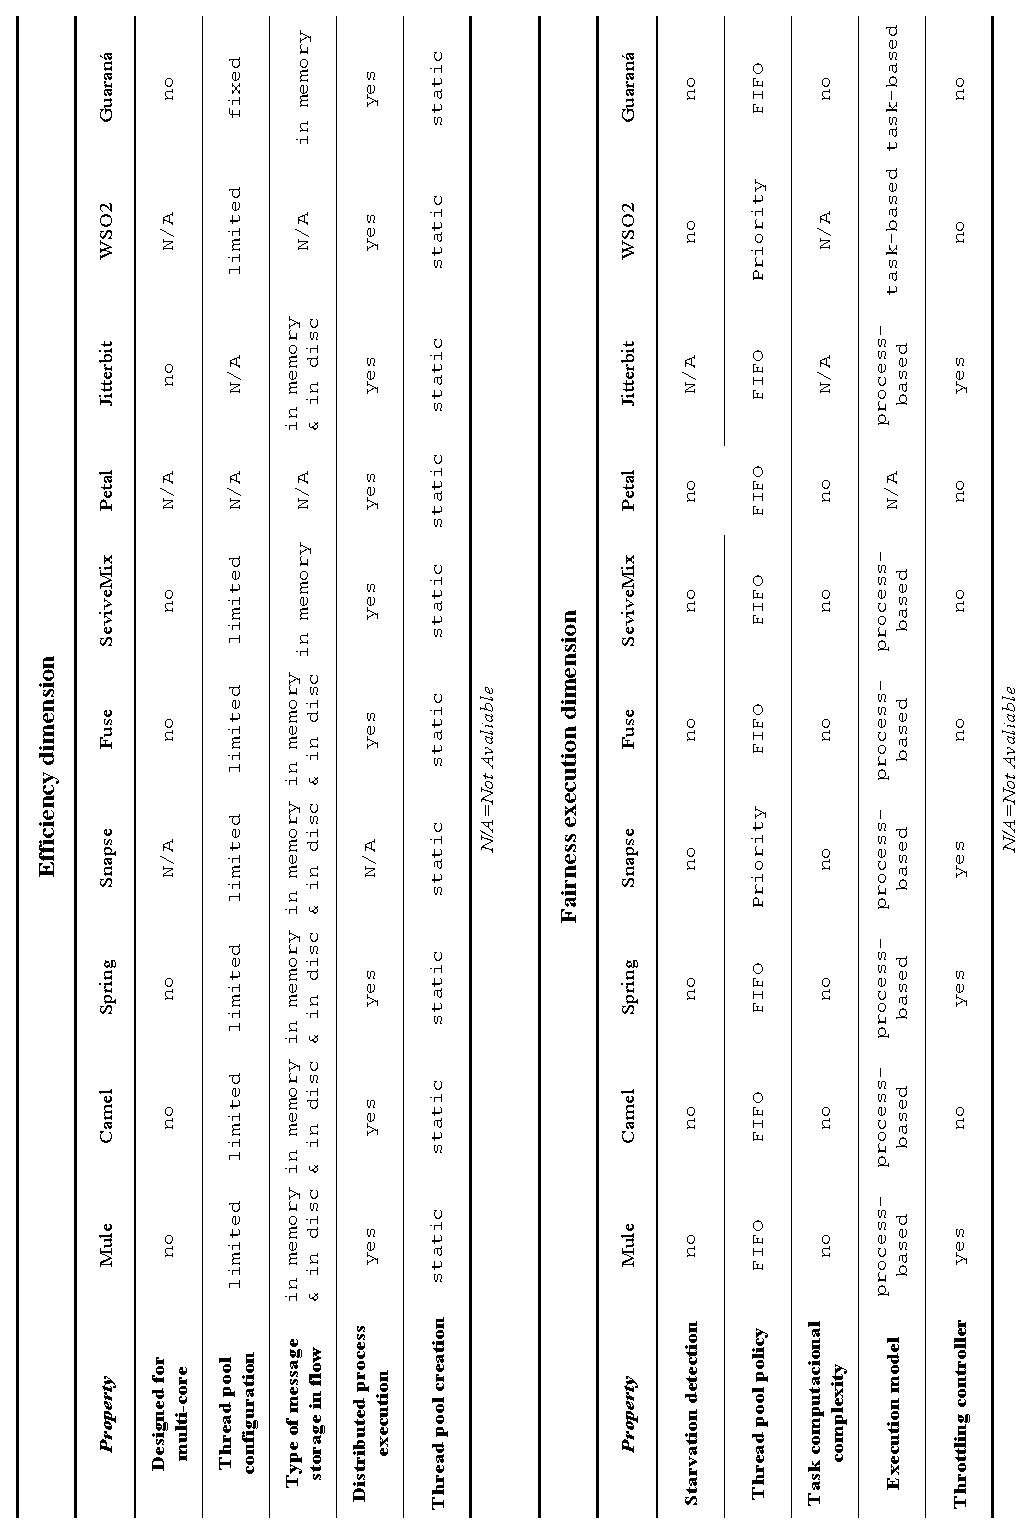
\includegraphics[scale=0.8]{./figs/table_dimensions_v.eps}
	%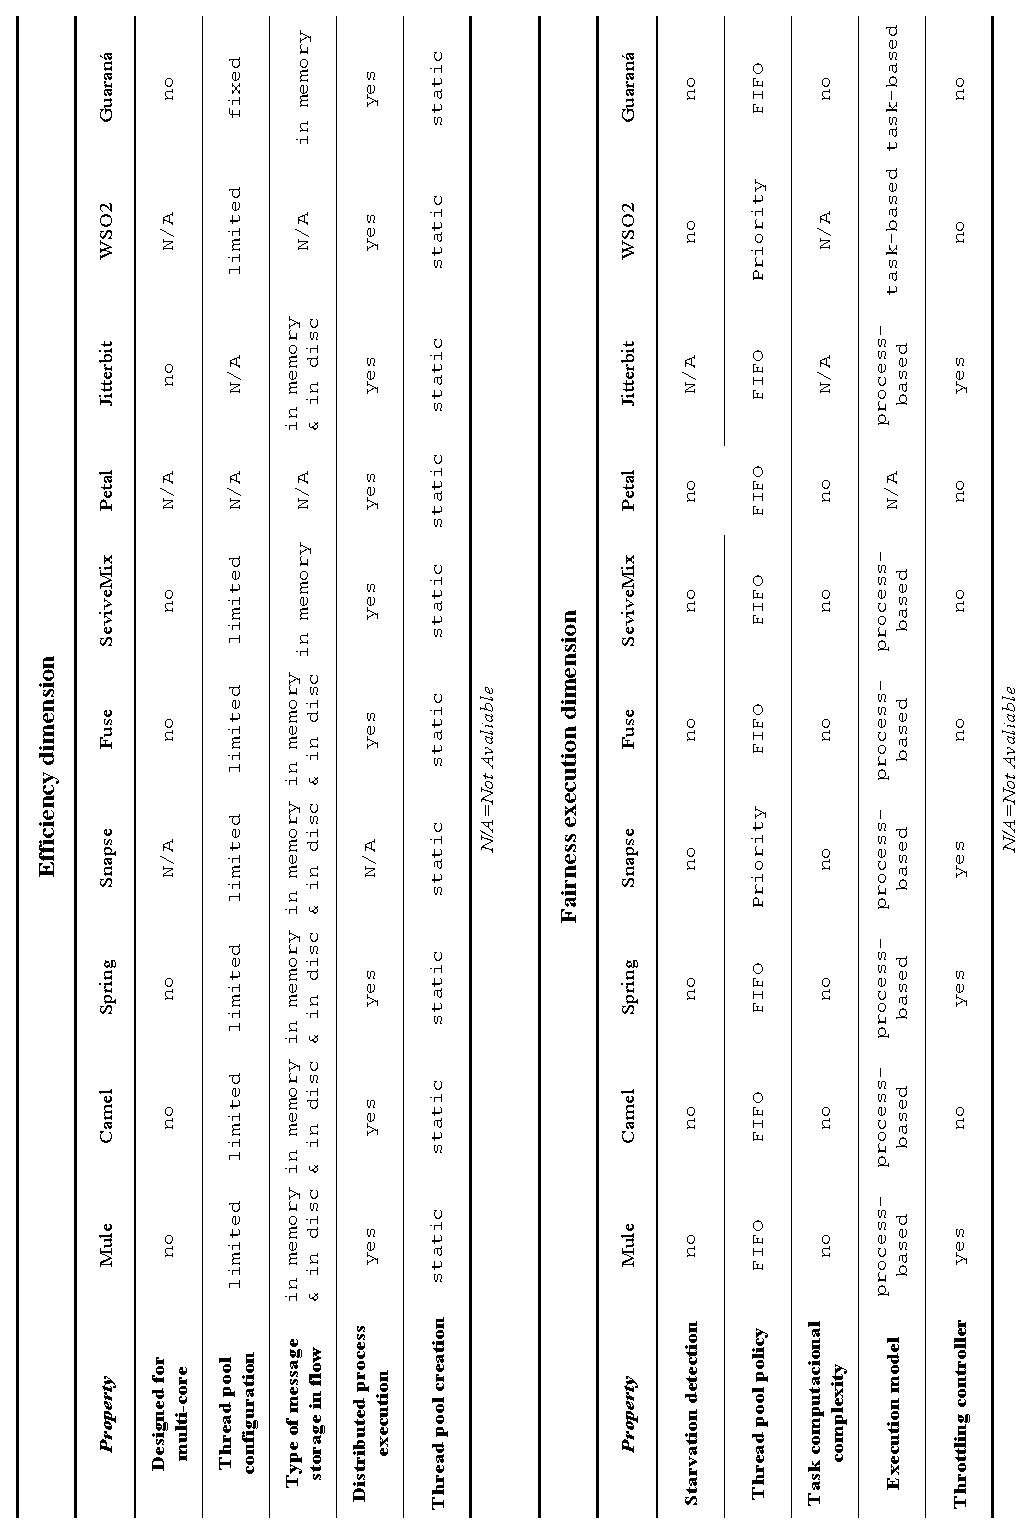
\includegraphics[width=\linewidth]{./figs/table_dimensions_v.eps}
	\label{tab:comparison}
\end{table*}

%==============================================================================
\subsubsection{Efficiency}
\label{subsubsec:comparasion_efficiency}
%============================================================================== 

\noindent

None of the integration platforms have their runtime system designed to take advantage of multi-core. Although, Mule, Camel and Jitterbit use some language resource for to implement the parallel programming, there not is information about proprieties of runtime systems that take advantage of physically tasks of an integration solution.

Every runtime systems have pools of threads which can increase or decrease the limited number of threads available to tasks, except Petals and Jitterbit, in which there is no information that allow us to evaluate them regarding this property; and Guaraná the provide a fixed pool of threads.

Mule, Camel, Spring Integration, Synapse, Fuse, ServiceMix and Jitterbit can deal with both common data, storing in memory, and big data, storing in disc. ServiceMix and WSO2, there is no information that allow us to evaluate them regarding this property, so we have assumed they, as well as Guaraná, store message only in memory.

The ability to distribute the execution of tasks amongst several virtual machines is present in every analysed runtime systems, except in Synapse, where there is no information that allow us to evaluate them regarding this property. 

None of these runtime systems is able to creation dynamically thread pool, optimising their task execution strategies from the analysis of the flow of messages in the integration solution. Petals, there is no information that allow us to evaluate it regarding this property, so we have assumed it do not provides creation dynamic thread pool.

%==============================================================================
\subsubsection{Fairness execution}
\label{subsubsec:comparasion_fairness}
%============================================================================== 
 
 \noindent

The capacity to detect tasks that are not executed within an accepted time frame is absent in every analysed runtime systems, except for Jitterbit, there is no information that allow us to evaluate it regarding this starvation detection property. Every analysed runtime systems chose FIFO heuristic as strategy for tasks scheduling, except Synapse and WSO2 have a strategy for distinguish tasks, in order to influence their scheduling, that is, priority based. 

None runtime systems considers the computational complexity of tasks to allocate threads, except for Jitterbit and WSO2, there is no information that allow us to evaluate them regarding this property, so we have assumed they not have considering the computational complexity of tasks to allocate threads.

Every runtime system implement process-based execution model, in which the runtime system controls process instances as a whole, except Guaraná and WSO2 which implement task-based execution model; and Petals, there is no information that allow us to evaluate them regarding this property, so we have assumed they adopt process-based execution model. 

Mule, Spring, Synapse and Jitterbit allow to control the rate of incoming messages on incoming ports; the others have not throttling controller.

%==============================================================================
\subsection{{Research Directions}}
\label{subsec:problems}
%==============================================================================

\noindent

In this section, we identify some research directions found out in this survey,  which facilitate the suitability of integration platforms in the cloud computing environment. Table~\ref{tab:problems} summarise the proprieties involved in these research directions. First, we  address the research directions regarding efficiency, after, about the research directions regarding of the fairness execution.

\begin{table}[hbtp]
	\centering
	%\caption{Issues to investigated.}
	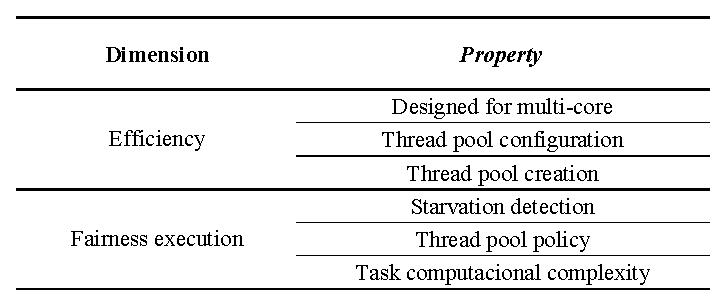
\includegraphics[scale=0.9]{./figs/issues.eps}
	%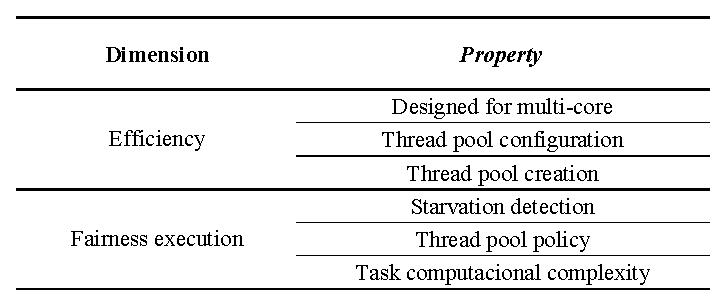
\includegraphics[width=\linewidth]{./figs/issues.eps}
\label{tab:problems}%
\end{table}%
%==============================================================================
\subsubsection{{Directions on Efficiency}}
\label{subsubsec:directions_efficiency}
%==============================================================================
Software engineers seek to develop algorithms that can take full advantage of multi-core design so that achieve a high level of parallelism and an overall high performance. The way the algorithms are written impact in the success of multi-core technology strongly~\cite{sethi2015}. Design multi-core is a property, which should be present in runtime systems bearing in mind that the technological advances already offers resources to extends the parallel program. For hardware, we can cite the modern technologies Graphics processing units (GPUs), which demand tens of thousands of concurrent threads to fully utilize the massive amount of processing resources~\cite{yoon2016}. GPUs hold great massively parallel computing capabilities, with potential for the acceleration of computationally intensive algorithms~\cite{tang2017}. 

Some works are shown promising proposals of thread pool configuration models, like the article of Nazeer et al.~\cite{nazeer2016}, which achieves good results in simulations, with the named Hybrid scheme to dynamically, which optimize a thread pool, based on predicting incoming request frequencies. Gleyzer et al.~\cite{gleyzer2017} propose a method allows dynamic thread pool sizing suitable for use in multi-threaded processing environment such as a distributed data grid. The method utilizes measurements of thread pool throughput and measurements of worker thread utilization in combination with analysis of prior thread pool resizing actions to determine whether to add or remove worker threads from a thread pool in a current resizing action. The method claims a rapid and responsive adjustment of thread pool size in response to changes in workload and processor availability. These works motivate us to deepen our research, so that the thread pool configuration of the runtime systems of the integration platforms occurs elastically, following the demand of processing the tasks and thus, using the computational resources more efficiently.

The research of Lee et al.~\cite{lee2011} shows better response time and CPU usage, by means prediction of the number of threads and thread pool management. Trendy exponential moving average (TEMA) scheme, proposed by Lee et al., adjusts the idle time out period and thread pool size to adapt the system to the changing environment. The article of Oh and Kim~\cite{oh2013} presents a history-based dynamic method (HisDyn), which minimizes throughput degradation, due to creation of threads, by means of estimation and maintenance of the number of threads needed for requests. HisDyn predicts the range of needed threads, through of the mean task arrival times and mean task processing times.

Bahadur et al.~\cite{bahadur2014} propose a thread pool system able of dynamic optimization thread pool size, according request frequencies, named Frequency Based Optimization Strategy (FBOS). After, Ashraf et al.~\cite{ashraf2016} present an extension of work of FBOS, namely Non-blocking Frequency Based Optimization Strategy with Automated Timers (NBFBOS with Automated Timers), which dynamically optimises thread pool, using of non-blocking synchronization primitives offering advantages of substantial scalability and liveliness. For all this, we believe that it is possible to find out to get optimised strategies to create threads at runtime to runtime systems of integration platforms.

%==============================================================================
\subsubsection{{Directions on Fairness execution}}
\label{subsubsec:directions_fairness}
%==============================================================================
Shah et al.~\cite{shah2017} argue that when starvation occurs it decreases response time and increases wait time to execution of requests and propose to explore the implementation of multiple thread pools based on a distribution of service times to avoid starvation and achieve concurrency of processing. Their analysis showed that proposed scheme is increases the response time and reduces the wait time. This research endorses the need and possibility of the runtime systems detecting starvation detection, therefore, the detection starvation is a potential field of study.

Tsai et al.~\cite{tsai2013} propose to optimize task scheduling and resource allocation using an improved differential evolution algorithm (IDEA), based on the proposed cost and time models on cloud computing environment. Elmougy et al.~\cite{elmougy2017} propose a novel hybrid task scheduling algorithm named (SRDQ) combining Shortest-Job-First (SJF) and Round Robin (RR) schedulers considering a dynamic variable task quantum. Singh et al.~\cite{singh2017} present a review of using meta-heuristics techniques for scheduling tasks in cloud computing, based on swarm intelligence and bio-inspired techniques and claim that it is possible to decide suitable approach for better schemes for scheduling according to the application. These works encourages us to pursue smarter policies to schedule tasks for the thread pools in the runtime systems of integration platforms.

Cordes et al.~\cite{cordes2011} claim that it is essential to balance the execution time of all tasks in a work flow of processing running in parallel in order to achieve the best possible utilization of computing resources. The proposed method by authors employs a cost model that allows incorporating differing execution times for loop iterations of the program due to the underlying heterogeneous platform. The consideration of execution time heterogeneity enables the in parallel approach to using each processing unit according to its performance characteristics in a system as well as the utilization of as many processing units as possible simultaneously.

The research of Sudarsanam et al.~\cite{sudarsanam2004} address the compatibility between resource and task by estimating the amount of resources that are needed for a reconfigurable architecture to suit task granularity. These studies point out that considering the computational complexity to be executed can lead to a better allocation of computational resources.

\doublespace
% Validation.tex
%==============================================================================
\section{Validation}
\label{sec:validation}
%==============================================================================

%-- Context
\noindent 

This section describes the model validated by means whose the solutions found for the implementation of a more efficient runtime system will be validated. 

%==============================================================================
\subsection{Statistical basis}
\label{subsec:statistical}
%==============================================================================

According to the Law of Large Numbers~\cite{hoeffding1961}, in a performance comparison of execution of applications between runtime systems, when the number of performance observations is infinite, then the performance distribution of each runtime system, as well as its quantitative features, can be accurately captured, becoming this comparison straightforward and accurate. However, in practice, the number of collected performance observations is limited, then it is necessary to introduce a quantitative indicator of confidence to judge whether a comparison result corresponds to a stochastic effect or whether it is significant enough to accept.

Usually, estimating confidences of performance evaluations use parametric statistic \textit{t}-statistics. However, in the context of runtime system performance, \textit{t}-statistics require the sample mean of the performance observations to be distributed normally, which must be guaranteed by either a normal performance distribution or a sufficiently large number of performance observations~\cite{sitthi2006}. For validation of the proposed runtime system, it will be used the Hierarchical Performance Testing (HPT) framework, based on non-parametric statistics, which provide a good quantitative estimate of the confidence and it is significantly more practical than standard \textit{t}-statistics, because it does not require to collect a large number of performance observations in order to achieve a normal distribution of sample mean.~\cite{chen2015}. 

%==============================================================================
\subsubsection{Non-parametric Hierarchical Performance Testing framework}
\label{subsubsec:statistical}
%==============================================================================

In HPT, performance samples of a runtime system $X$ and of a runtime system $Y$ can be represented by performance matrices $S_{X}={\left [ x_{i,j} \right ]}_{m \ast  n}$ and  $S_{Y}={\left [ y_{i,j} \right ]}_{m \ast  n}$, respectively, where $n$ is a total number benchmark applications and $m$ is a total number of repetitions of execution of the application. So, the performance scores of $X$ and $Y$ at their $j-th$ runs on the $i-th$ benchmark is $x_{i,j}$ and  $y_{i,j}$ respectively. For the corresponding rows of $S_{X}$ and $S_{Y}$.

HPT establishes as the null hypothesis and the alternative hypothesis of Statistical Hypothesis Test (SHT):

The Wilcoxon Rank-Sum Test\cite{{wilcoxon1992} is used to investigate whether the difference between the performance score of $X$ and $Y$ is significant enough. The steps of Wilcoxon Rank-Sum Test are described as following:
\begin{itemize}
\item 
\end{itemize}

\doublespace
% Schedule.tex
%==============================================================================
\section{Schedule}
\label{sec:schedule}
%==============================================================================

\noindent 

This section presents the schedule of activities for the development of this doctoral research project, starting in April of 2016 and ending in March 2020, totalling a period of 48 months.
Table~\ref{tab:schedule1} presents the planning of the academic training activities and the planning of the research activities.

\begin{table*}[!htbp]
	\centering
	\caption{Schedule of activities.}
    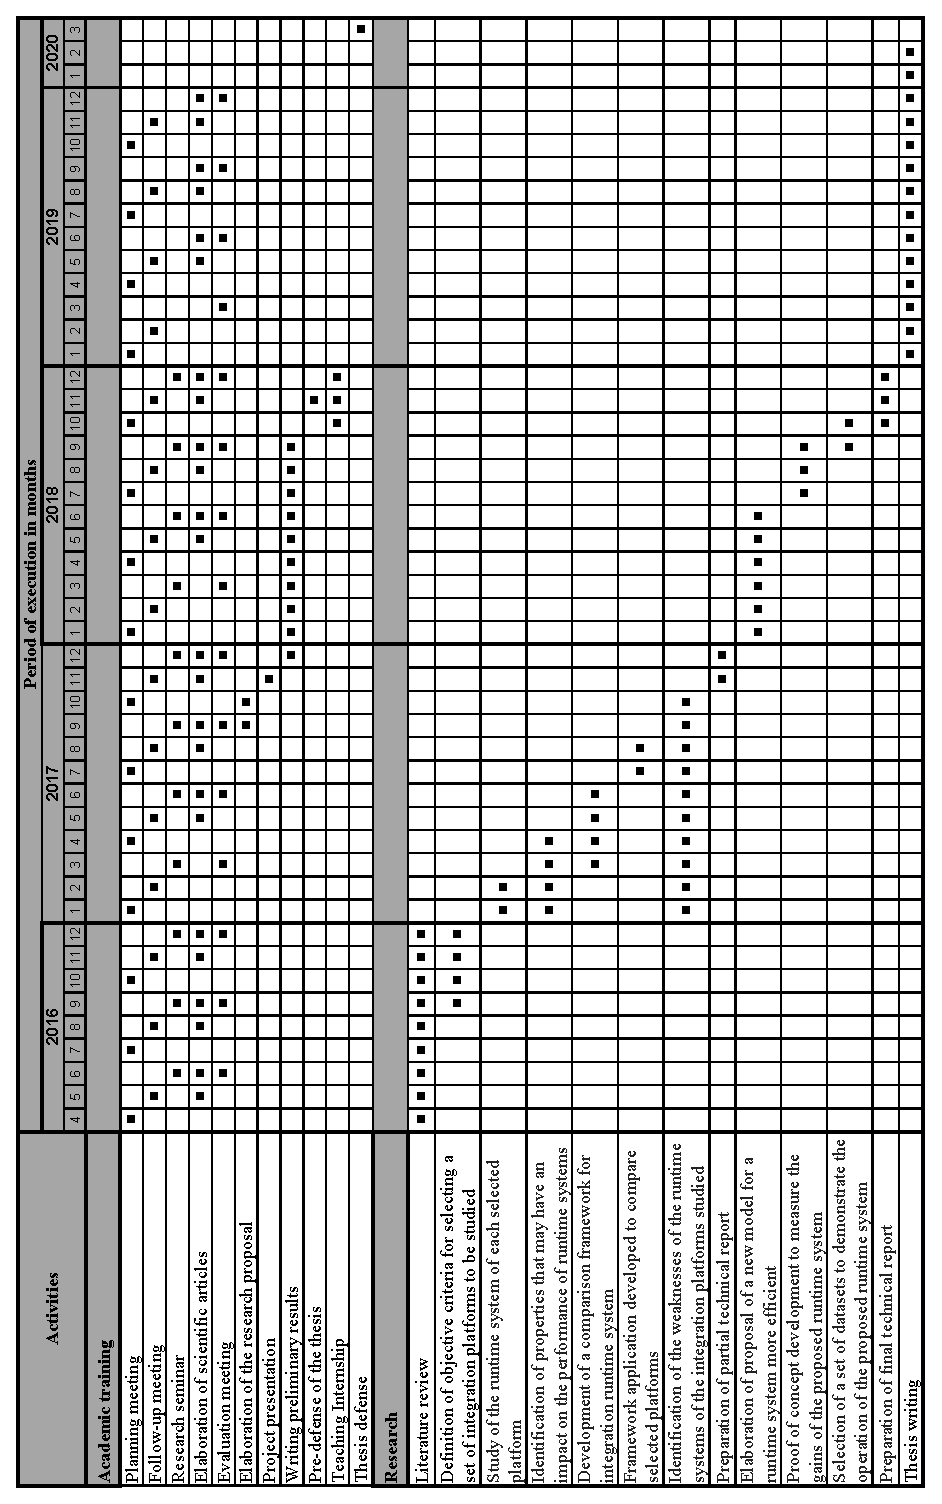
\includegraphics[scale=0.8]{./figs/chrono.eps}
	%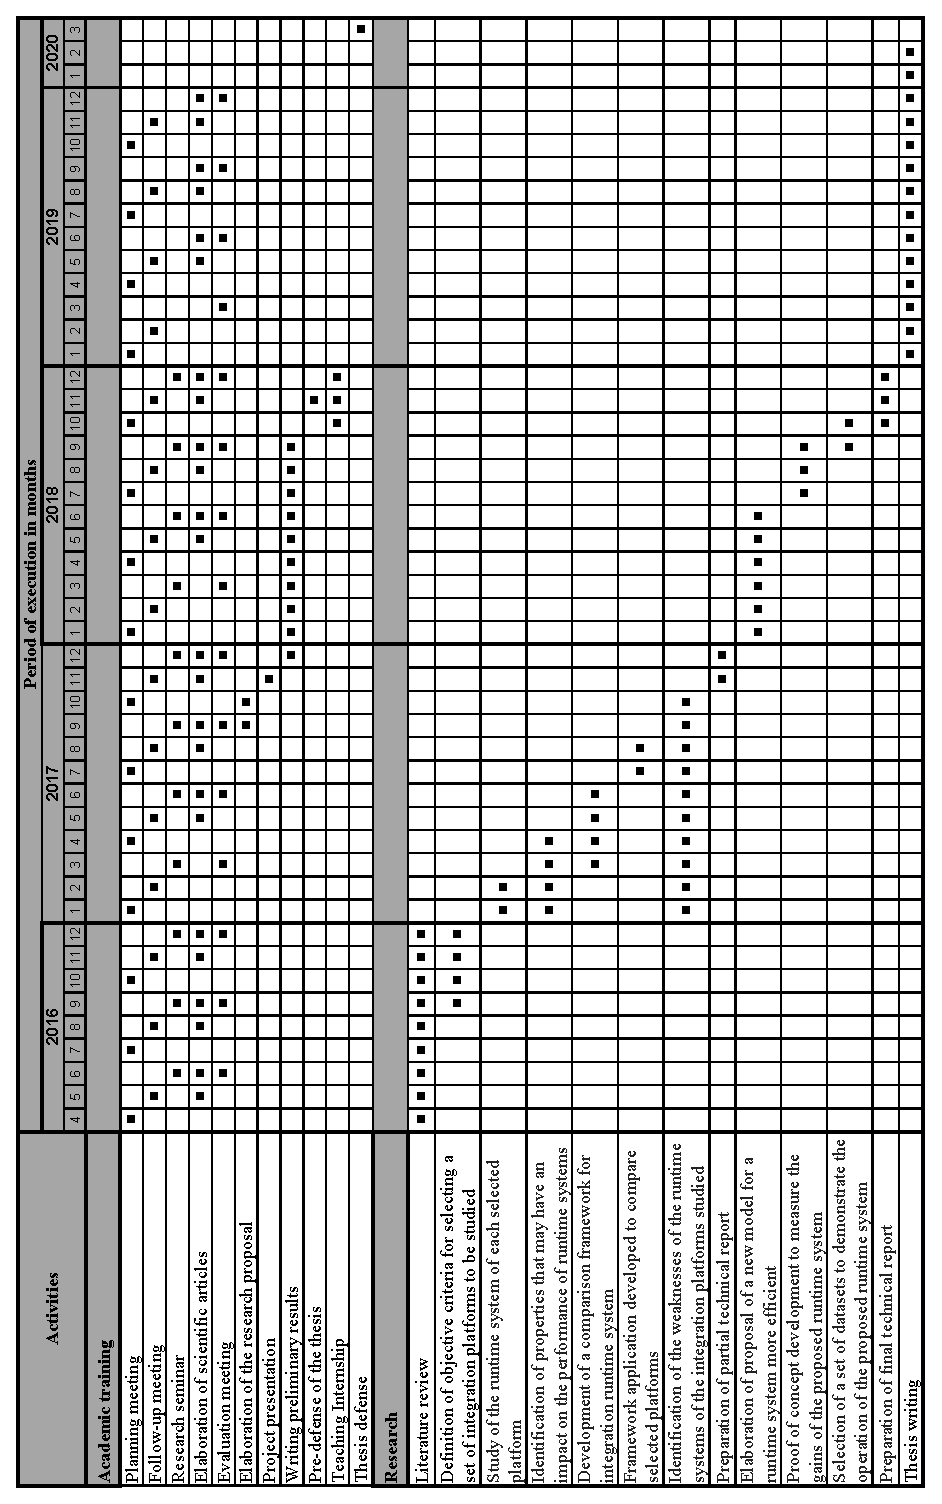
\includegraphics[width=\linewidth]{./figs/chrono.eps}
	\label{tab:schedule1}
\end{table*}
\doublespace
% Conclusions.tex
%==============================================================================
\section{Conclusions}
\label{sec:conclusions}
%==============================================================================

\noindent
Cloud computing has offered several services to companies, which open the chance to leverage their business processes. These services frequently require the integration of different applications, which compose the software ecosystem. Thus, the companies need to rely on integration runtime systems tools that provide appropriate performance.

Integration platforms are specialised software tools that allow keeping information on all these systems consistent and synchronised. Usually, an integration platform is composed of a domain-specific language, a development toolkit, a runtime system and monitoring tools. The runtime system is responsible for running integration solutions and therefore, its performance most often drives the decision of companies to chose an integration platform.

In this article, we presented a survey about runtime systems, extracting proprieties, which that can have an impact on the performance of the runtime system.  Such properties allow to analyse runtime systems,.focusing on performance. These properties make up two dimensions: efficiency and fairness execution. Efficiency focuses on the efficient message processing within an integration solution and fairness execution focuses on the fair execution of tasks within an integration solution. 

We compare the runtime system of ten different integration platforms and it was possible to identify that the runtime systems have advanced regarding efficiency, such as, most of them allow that the number of threads in a thread pool can increase automatically during runtime until a threshold defined at design time is reached; most of them store messages in memory and on disk; everyone are able to distribute the processing. On the other hand, none has designed to take advantage of multi-core and none is able to creation dynamically thread pool.

However, the platforms have few functionalities that allow the fair execution of the tasks. This can be concluded due to runtime systems: none is able to detect tasks that have been waiting for a long time to be executed, that is, starvation detect; most of them uses basic heuristics as scheduling policy to tasks; none knows their computational complexity of these tasks; most of them adopts the execution model process-based; only the smallest part of them has some kind of throttling controller for to limit the incoming rate.

Based on these findings, we will consider as research directions in order to achieve better performance results of the runtime systems of the integration platforms, the following proprieties: designed for multi-core, thread pool configuration, thread pool creation of efficiency dimension and starvation detection, thread pool policy, task complexity of fairness execution dimension. For these issues, we find, in the literature, several approaches that motivate us to deepen our research.


\pagebreak

% This includes all references from the BibTeX file in the bibliography
\nocite{*}

\begin{spacing}{1}
  \bibliographystyle{plain}
  \bibliography{./bib/Bibliography}
\end{spacing}

\end{document}
